%% Преамбула TeX-файла

% 1. Стиль и язык
\documentclass[utf8x, 12pt]{G7-32} % Стиль (по умолчанию будет 14pt)

% Остальные стандартные настройки убраны в preamble.inc.tex.
\usepackage{cmap} % Улучшенный поиск русских слов в полученном pdf-файле
\usepackage[T2A]{fontenc} % Поддержка русских букв
\usepackage[utf8]{inputenc} % Кодировка utf8
\usepackage[english,russian]{babel} % Языки: русский, английский
%\usepackage{pscyr} % Нормальные шрифты
\usepackage{enumitem}

\usepackage[normalem]{ulem}
\usepackage{cancel}
\usepackage{float}
\usepackage[14pt]{extsizes}

\usepackage{caption}
\captionsetup{labelsep=endash}
\captionsetup[figure]{name={Рисунок}}

\usepackage{amsmath}

\usepackage{geometry}
\geometry{left=30mm}
\geometry{right=15mm}
\geometry{top=20mm}
\geometry{bottom=20mm}

\usepackage{titlesec}
\titleformat{\section}
	{\normalsize\bfseries}
	{\thesection}
	{1em}{}
\titlespacing*{\chapter}{0pt}{-30pt}{8pt}
\titlespacing*{\section}{\parindent}{*4}{*4}
\titlespacing*{\subsection}{\parindent}{*4}{*4}

\usepackage{setspace}
\onehalfspacing % Полуторный интервал

\frenchspacing
\usepackage{indentfirst} % Красная строка

\usepackage{titlesec}
\titleformat{\chapter}{\LARGE\bfseries}{\thechapter}{20pt}{\LARGE\bfseries}
\titleformat{\section}{\Large\bfseries}{\thesection}{20pt}{\Large\bfseries}

\usepackage{listings}
\usepackage{xcolor}

% Для листинга кода:
\lstset{ %
	language=c++,   					% выбор языка для подсветки	
	basicstyle=\small\sffamily,			% размер и начертание шрифта для подсветки кода
	numbers=left,						% где поставить нумерацию строк (слева\справа)
	%numberstyle=,					% размер шрифта для номеров строк
	stepnumber=1,						% размер шага между двумя номерами строк
	numbersep=5pt,						% как далеко отстоят номера строк от подсвечиваемого кода
	frame=single,						% рисовать рамку вокруг кода
	tabsize=4,							% размер табуляции по умолчанию равен 4 пробелам
	captionpos=t,						% позиция заголовка вверху [t] или внизу [b]
	breaklines=true,					
	breakatwhitespace=true,				% переносить строки только если есть пробел
	escapeinside={\#*}{*)},				% если нужно добавить комментарии в коде
	backgroundcolor=\color{white},
}

\usepackage{pgfplots}
\usetikzlibrary{datavisualization}
\usetikzlibrary{datavisualization.formats.functions}

\usepackage{graphicx}
\newcommand{\img}[3] {
	\begin{figure}[h!]
		\center{\includegraphics[height=#1]{inc/img/#2}}
		\caption{#3}
		\label{img:#2}
	\end{figure}
}
\newcommand{\boximg}[3] {
	\begin{figure}[h]
		\center{\fbox{\includegraphics[height=#1]{inc/img/#2}}}
		\caption{#3}
		\label{img:#2}
	\end{figure}
}

\usepackage[justification=centering]{caption} % Настройка подписей float объектов

\usepackage[unicode,pdftex]{hyperref} % Ссылки в pdf
\hypersetup{hidelinks}

\usepackage{csvsimple}

\setlength{\parindent}{1.25cm}

\makeatletter
\renewcommand\@biblabel[1]{#1.}
\makeatother

\newcommand{\code}[1]{\texttt{#1}}


% Настройки листингов.
\ifPDFTeX
% 8 Листинги

\usepackage{listings}

% Значения по умолчанию
\lstset{
  basicstyle= \footnotesize,
  breakatwhitespace=true,% разрыв строк только на whitespacce
  breaklines=true,       % переносить длинные строки
%   captionpos=b,          % подписи снизу -- вроде не надо
  inputencoding=koi8-r,
  numbers=left,          % нумерация слева
  numberstyle=\footnotesize,
  showspaces=false,      % показывать пробелы подчеркиваниями -- идиотизм 70-х годов
  showstringspaces=false,
  showtabs=false,        % и табы тоже
  stepnumber=1,
  tabsize=4,              % кому нужны табы по 8 символов?
  frame=single,
  xleftmargin=2.4em,
  framexleftmargin=2em
}

% Стиль для псевдокода: строчки обычно короткие, поэтому размер шрифта побольше
\lstdefinestyle{pseudocode}{
  basicstyle=\small,
  keywordstyle=\color{black}\bfseries\underbar,
  language=Pseudocode,
  numberstyle=\footnotesize,
  commentstyle=\footnotesize\it
}

% Стиль для обычного кода: маленький шрифт
\lstdefinestyle{realcode}{
  basicstyle=\scriptsize,
  numberstyle=\footnotesize
}

% Стиль для коротких кусков обычного кода: средний шрифт
\lstdefinestyle{simplecode}{
  basicstyle=\footnotesize,
  numberstyle=\footnotesize
}

% Стиль для BNF
\lstdefinestyle{grammar}{
  basicstyle=\footnotesize,
  numberstyle=\footnotesize,
  stringstyle=\bfseries\ttfamily,
  language=BNF
}

% Определим свой язык для написания псевдокодов на основе Python
\lstdefinelanguage[]{Pseudocode}[]{Python}{
  morekeywords={each,empty,wait,do},% ключевые слова добавлять сюда
  morecomment=[s]{\{}{\}},% комменты {а-ля Pascal} смотрятся нагляднее
  literate=% а сюда добавлять операторы, которые хотите отображать как мат. символы
    {->}{\ensuremath{$\rightarrow$}~}2%
    {<-}{\ensuremath{$\leftarrow$}~}2%
    {:=}{\ensuremath{$\leftarrow$}~}2%
    {<--}{\ensuremath{$\Longleftarrow$}~}2%
}[keywords,comments]

% Свой язык для задания грамматик в BNF
\lstdefinelanguage[]{BNF}[]{}{
  morekeywords={},
  morecomment=[s]{@}{@},
  morestring=[b]",%
  literate=%
    {->}{\ensuremath{$\rightarrow$}~}2%
    {*}{\ensuremath{$^*$}~}2%
    {+}{\ensuremath{$^+$}~}2%
    {|}{\ensuremath{$|$}~}2%
}[keywords,comments,strings]

% Подписи к листингам на русском языке.
\renewcommand\lstlistingname{Листинг}
\renewcommand\lstlistlistingname{Листинги}

\else
\usepackage{local-minted}

\fi

% Стиль титульного листа и заголовки
% 
\begin{titlepage}
	\newgeometry{pdftex, left=2cm, right=2cm, top=2.5cm, bottom=2.5cm}
	\fontsize{12pt}{12pt}\selectfont
	\noindent \begin{minipage}{0.15\textwidth}
		
\includegraphics[width=\linewidth]{inc/img/b_logo.jpg}
	\end{minipage}
	\noindent\begin{minipage}{0.9\textwidth}\centering
		\textbf{Министерство науки и высшего образования Российской Федерации}\\
		\textbf{Федеральное государственное бюджетное образовательное учреждение высшего образования}\\
		\textbf{«Московский государственный технический университет имени Н.Э.~Баумана}\\
		\textbf{(национальный исследовательский университет)»}\\
		\textbf{(МГТУ им. Н.Э.~Баумана)}
	\end{minipage}
	
	\noindent\rule{18cm}{3pt}
	\newline\newline
	\noindent ФАКУЛЬТЕТ $\underline{\text{«Информатика и системы управления»~~~~~~~~~~~~~~~~~~~~~~~~~~~~~~~~~~~~~~~~~~~~~~~~~~~~~~~}}$ \newline\newline
	\noindent КАФЕДРА $\underline{\text{«Программное обеспечение ЭВМ и информационные технологии»~~~~~~~~~~~~~~~~~~~~~~~}}$\newline\newline\newline\newline\newline\newline\newline
	
	
	\begin{center}
		\Large\textbf{Отчет по лабораторной работе №4}
		\Large\textbf {по курсу "Анализ алгоритмов"}
	\end{center}
	\noindent\textbf{Тема} $\underline{\text{~~Параллельные вычисления на основе нативных потоков~~~~~~~~~~~~~~~~~~~~~~~~~~~~~~~~~~~~~~~~~}}$\newline\newline\newline
	\noindent\textbf{Студент} $\underline{\text{~~Золотухин А.В.~~~~~~~~~~~~~~~~~~~~~~~~~~~~~~~~~~~~~~~~~~~~~~~~~~~~~~~~~~~~~~~~~~~~~~~~~~~~~~~~~~~~~~~~~}}$\newline\newline
	\noindent\textbf{Группа} $\underline{\text{~~ИУ7-54Б~~~~~~~~~~~~~~~~~~~~~~~~~~~~~~~~~~~~~~~~~~~~~~~~~~~~~~~~~~~~~~~~~~~~~~~~~~~~~~~~~~~~~~~~~~~~~~~~~}}$\newline\newline
	\noindent\textbf{Оценка (баллы)} $\underline{\text{~~~~~~~~~~~~~~~~~~~~~~~~~~~~~~~~~~~~~~~~~~~~~~~~~~~~~~~~~~~~~~~~~~~~~~~~~~~~~~~~~~~~~~~~~~~~~~~~~~~}}$\newline\newline
	\noindent\textbf{Преподаватели} $\underline{\text{~~Волкова Л.Л., Строганов Ю.В.~~~~~~~~~~~~~~~~~~~~~~~~~~~~~~~~~~~~~~~~~~~~~~~~~~~~~~~~~~~}}$\newline
	
	\begin{center}
		\vfill
		Москва~---~\the\year
		~г.
	\end{center}
	\restoregeometry
\end{titlepage}




\begin{document}

\begin{titlepage}
	\newgeometry{pdftex, left=2cm, right=2cm, top=2.5cm, bottom=2.5cm}
	\fontsize{12pt}{12pt}\selectfont
	\noindent \begin{minipage}{0.15\textwidth}
		
\includegraphics[width=\linewidth]{inc/img/b_logo.jpg}
	\end{minipage}
	\noindent\begin{minipage}{0.9\textwidth}\centering
		\textbf{Министерство науки и высшего образования Российской Федерации}\\
		\textbf{Федеральное государственное бюджетное образовательное учреждение высшего образования}\\
		\textbf{«Московский государственный технический университет имени Н.Э.~Баумана}\\
		\textbf{(национальный исследовательский университет)»}\\
		\textbf{(МГТУ им. Н.Э.~Баумана)}
	\end{minipage}
	
	\noindent\rule{18cm}{3pt}
	\newline\newline
	\noindent ФАКУЛЬТЕТ $\underline{\text{«Информатика и системы управления»~~~~~~~~~~~~~~~~~~~~~~~~~~~~~~~~~~~~~~~~~~~~~~~~~~~~~~~}}$ \newline\newline
	\noindent КАФЕДРА $\underline{\text{«Программное обеспечение ЭВМ и информационные технологии»~~~~~~~~~~~~~~~~~~~~~~~}}$\newline\newline\newline\newline\newline\newline\newline
	
	
	\begin{center}
		\Large\textbf{Отчет по лабораторной работе №4}
		\Large\textbf {по курсу "Анализ алгоритмов"}
	\end{center}
	\noindent\textbf{Тема} $\underline{\text{~~Параллельные вычисления на основе нативных потоков~~~~~~~~~~~~~~~~~~~~~~~~~~~~~~~~~~~~~~~~~}}$\newline\newline\newline
	\noindent\textbf{Студент} $\underline{\text{~~Золотухин А.В.~~~~~~~~~~~~~~~~~~~~~~~~~~~~~~~~~~~~~~~~~~~~~~~~~~~~~~~~~~~~~~~~~~~~~~~~~~~~~~~~~~~~~~~~~}}$\newline\newline
	\noindent\textbf{Группа} $\underline{\text{~~ИУ7-54Б~~~~~~~~~~~~~~~~~~~~~~~~~~~~~~~~~~~~~~~~~~~~~~~~~~~~~~~~~~~~~~~~~~~~~~~~~~~~~~~~~~~~~~~~~~~~~~~~~}}$\newline\newline
	\noindent\textbf{Оценка (баллы)} $\underline{\text{~~~~~~~~~~~~~~~~~~~~~~~~~~~~~~~~~~~~~~~~~~~~~~~~~~~~~~~~~~~~~~~~~~~~~~~~~~~~~~~~~~~~~~~~~~~~~~~~~~~}}$\newline\newline
	\noindent\textbf{Преподаватели} $\underline{\text{~~Волкова Л.Л., Строганов Ю.В.~~~~~~~~~~~~~~~~~~~~~~~~~~~~~~~~~~~~~~~~~~~~~~~~~~~~~~~~~~~}}$\newline
	
	\begin{center}
		\vfill
		Москва~---~\the\year
		~г.
	\end{center}
	\restoregeometry
\end{titlepage}


\pagenumbering{arabic}
\setcounter{page}{2}
\frontmatter % выключает нумерацию ВСЕГО; здесь начинаются ненумерованные главы: реферат, введение, глоссарий, сокращения и прочее.

%\maketitle %создает титульную страницу
% \afterpage{\blankpage}\afterpage{\blankpage}\afterpage{\blankpage}
% пропущены страницы под тз и план (у меня их 2 тз и 1 план, итого 3, вам надо пропустить столько, сколько страниц у вас в тз и плане)


%\listoffigures                         % Список рисунков

%\listoftables                          % Список таблиц

%\NormRefs % Нормативные ссылки 
% Команды \breakingbeforechapters и \nonbreakingbeforechapters
% управляют разрывом страницы перед главами.
% По-умолчанию страница разрывается.

% \Referat
%\begin{abstract}

    Отчет содержит \pageref{LastPage}\,стр.%
    \ifnum \totfig >0
    , \totfig~рис.%
    \fi
    \ifnum \tottab >0
    , \tottab~табл.%
    \fi
    %
    \ifnum \totbib >0
    , \totbib~источн.%
    \fi
    %
    \ifnum \totapp >0
    , \totapp~прил.%
    \else
    .%
    \fi


%\end{abstract}

%%% Local Variables: 
%%% mode: latex
%%% TeX-master: "rpz"
%%% End: 

% \nobreakingbeforechapters
% \breakingbeforechapters

\tableofcontents

% \printnomenclature % Автоматический список сокращений

\Introduction

Цель данной лабораторной работы --- реализовать в виде программы аналог шифровальной машины ``Энигма''.

Информацию для разных целей пытались засекречивать с помощью шифрования на протяжении всей истории человечества. Шифр --- это множество обратимых преобразований открытого текста, проводимых с целью его защиты от несанкционированного использования. Одним из таких шифров является энигма.

В рамках выполнения лабораторной работы необходимо решить следующие задачи: 
\begin{itemize}
	\item описать алгоритм шифровальной машины Энигма;
	\item реализовать алгоритм.
\end{itemize}

\mainmatter % это включает нумерацию глав и секций в документе ниже

\chapter{Аналитический раздел}
\label{cha:analysis}

\section{Алгоритм шифрования DES}

DES (Data Encryption Standard) - это симметричный шифровальный алгоритм, разработанный в 1970-х годах, который использует блочное шифрование с фиксированной длиной блока в 64 бита. Вот основные шаги и логика работы DES:

1. Начальная перестановка (Initial Permutation):
Исходный текст (64 бита) проходит через начальную перестановку, где биты переставляются в определенном порядке согласно предопределенной таблице перестановок.

2. Раунды (Rounds):
DES состоит из 16 раундов шифрования, каждый из которых включает несколько шагов:
\begin{itemize}
	\item Расширение (Expansion): 32-битный входной блок расширяется до 48 бит путем перестановки и дублирования некоторых битов.
	\item Ключ раунда (Round Key): к 48-битному расширенному блоку применяется 48-битный ключ раунда, полученный из основного ключа DES.
	\item Скремблирование (Substitution): 48-битный блок проходит через S-блоки (Substitution-boxes), которые заменяют блоки по 6 бит на блоки по 4 бита с использованием заранее определенных таблиц замен.
	\item Перестановка (Permutation):  после замены, полученный блок по 32 бита проходит через таблицу перестановки, которая перемешивает биты в блоке.
	\item Обработка ключа (Key Mixing): к полученному блоку применяется операция XOR с ключом раунда для обеспечения взаимодействия ключа и данных.
\end{itemize}

3. Последняя перестановка (Final Permutation):
После 16 раундов, 64-битный блок проходит через последнюю перестановку, обратную начальной перестановке, чтобы получить зашифрованный текст.

Основным элементом DES является ключ, который состоит из 56 бит, и который используется для генерации ключей раунда. Ключ разбивается на две половины, и каждая половина сдвигается влево на определенное количество бит в зависимости от номера раунда. Затем, из полученных половинок формируется ключ раунда.

Таким образом, DES использует комбинацию перестановок, замен и операций XOR для шифрования данных. Эти шаги повторяются 16 раз, в каждом раунде используется уникальный ключ. Результат - зашифрованный блок данных, который без знания правильного ключа практически невозможно расшифровать.

Для DES рекомендовано несколько режимов:

\begin{itemize}
	\item ECB (англ. electronic code book) --- режим «электронной кодовой книги» (простая замена);
	\item CBC (англ. cipher block chaining) --- режим сцепления блоков;
	\item CFB (англ. cipher feed back) --- режим обратной связи по шифротексту;
	\item OFB (англ. output feed back) --- режим обратной связи по выходу.
\end{itemize}

\section*{Вывод}
В данном разделе был рассмотрен алгоритм симметричного шифрования DES.
\chapter{Конструкторский раздел}
\label{cha:design}

В данном разделе будет представлена схема алгоритма шифрования DES.

\section{Алгоритм шифрования DES}

На рисунке \ref{fig:des01} изображена обобщенная схема шифрования DES.


\begin{figure}[H]
	\centering
	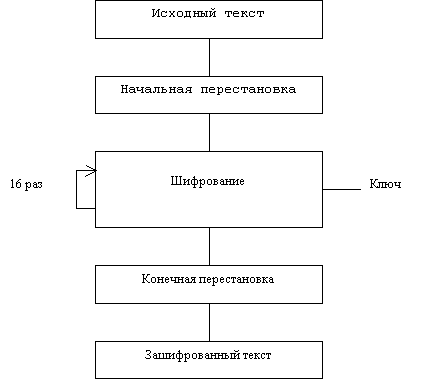
\includegraphics[width=0.7\linewidth]{img/des_01}
	\caption{Обобщенная схема шифрования DES}
	\label{fig:des01}
\end{figure}

На рисунке \ref{fig:des3} изображена структура алгоритма DES.

\begin{figure}[H]
	\centering
	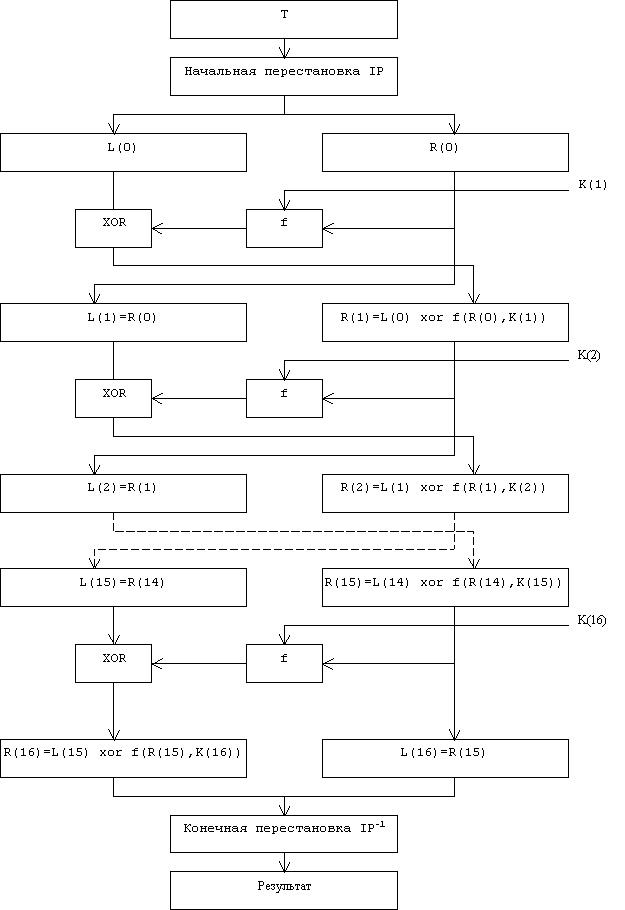
\includegraphics[width=0.7\linewidth]{img/des_3}
	\caption{Структура алгоритма DES}
	\label{fig:des3}
\end{figure}

На рисунке \ref{fig:des4} схематически изображено вычисление функции $f(R(i-1), K(i))$.

\begin{figure}[H]
	\centering
	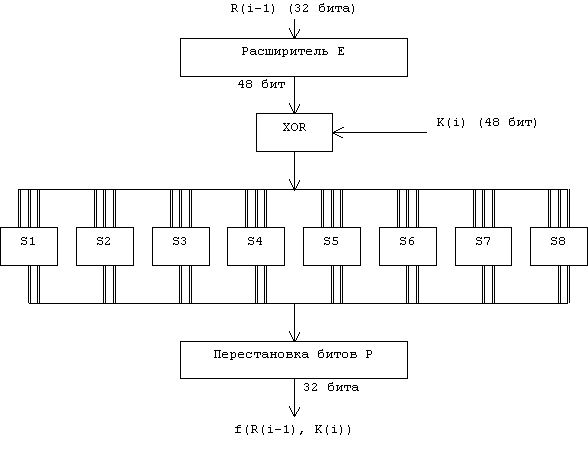
\includegraphics[width=0.7\linewidth]{img/des_4}
	\caption{Вычисление функции $f(R(i-1), K(i))$}
	\label{fig:des4}
\end{figure}


\section*{Вывод}
В данном разделе были приведены схемы алгоритма шифрования DES.



\chapter{Технологический раздел}
\label{cha:impl}

\section{Средства реализации}

В качестве языка программирования для реализации данной лабораторной работы использовался язык программирования С++ \cite{cplusplus}, так как он позволяет работать с файлами и массивами. В качестве среды разработки использовалась Visual Studio Code \cite{vscode}.

\section{Реализация алгоритмов}

В листингах \ref{code:rotor}--\ref{code:enigma} представлена реализация алгоритма шифрования DES.

\begin{lstlisting}[label=code:rotor,caption=Функция шифрования файла]
int FileEncryption::cipher(string input, string output, bool mode)
{
	ifstream ifile;
	ofstream ofile;
	ui64 buffer;
	
	if(input.length()  < 1) 
	ifile = ifstream(stdin);
	else
	ifile.open(input, ios::binary | ios::in | ios::ate);
	
	if(output.length() < 1) 
	ofile = ofstream(stdout);
	else
	ofile.open(output, ios::binary | ios::out);
	
	ui64 size = ifile.tellg();
	ifile.seekg(0, ios::beg);
	
	ui64 block = size / 8;
	if(mode) block--;
	
	for(ui64 i = 0; i < block; i++)
	{
		ifile.read((char*) &buffer, 8);
		if (mode)
		buffer = des.decrypt(buffer);
		else
		buffer = des.encrypt(buffer);
		
		ofile.write((char*) &buffer, 8);
	}
	
	if(mode == false)
	{
		ui8 padding = 8 - (size % 8);
		
		if (padding == 0)
		padding  = 8;
		
		buffer = (ui64) 0;
		if(padding != 8)
		ifile.read((char*) &buffer, 8 - padding);
		
		ui8 shift = padding * 8;
		buffer <<= shift;
		buffer  |= (ui64) 0x0000000000000001 << (shift - 1);
		
		buffer = des.encrypt(buffer);
		ofile.write((char*) &buffer, 8);
	}
	else
	{
		ifile.read((char*) &buffer, 8);
		buffer = des.decrypt(buffer);
		
		ui8 padding = 0;
		
		while(!(buffer & 0x00000000000000ff))
		{
			buffer >>= 8;
			padding++;
		}
		
		buffer >>= 8;
		padding++;
		
		if(padding != 8)
		ofile.write((char*) &buffer, 8 - padding);
	}
	
	ifile.close();
	ofile.close();
	return 0;
}
\end{lstlisting}

\begin{lstlisting}[label=code:reflector,caption=Функция шифратора]
ui64 DES::des(ui64 block, bool mode)
{
	block = ip(block);
	
	ui32 L = (ui32) (block >> 32) & L64_MASK;
	ui32 R = (ui32) (block & L64_MASK);
	
	for (ui8 i = 0; i < 16; i++)
	{
		ui32 F;
		if (mode)
		F = f(R, sub_key[15 - i]);
		else
		F = f(R, sub_key[i]);
		ui32 temp = R;
		R = L ^ F;
		L = temp;
	}
	
	block = (((ui64) R) << 32) | (ui64) L;
	return fp(block);
}
\end{lstlisting}

\begin{lstlisting}[label=code:enigma,caption=Функция Фейстеля]
ui32 DES::f(ui32 R, ui64 k)
{
	ui64 s_input = 0;
	for (ui8 i = 0; i < 48; i++)
	{
		s_input <<= 1;
		s_input |= (ui64) ((R >> (32-EXPANSION[i])) & LB32_MASK);
	}
	s_input = s_input ^ k;
	ui32 s_output = 0;
	for (ui8 i = 0; i < 8; i++)
	{
		char s = (s_input >> (42 - 6 * i)) & 0x3f;
		char row = ((s >> 4) & 0b10) | s & 1;
		char column = (s >> 1) & 0b1111;
		
		s_output <<= 4;
		s_output |= (ui32) (SBOX[i][16*row + column] & 0x0f);
	}
	
	ui32 f_result = 0;
	for (ui8 i = 0; i < 32; i++)
	{
		f_result <<= 1;
		f_result |= (s_output >> (32 - PBOX[i])) & LB32_MASK;
	}
	
	return f_result;
}
\end{lstlisting}

\section{Тестирование реализации алгоритма}

Было проведено тестирование на следующих входных данных:

1. Входящая последовательность байтов:

D09BD0B8D0BDD0B5D0B9D0BDD18BD0B9

Зашифрованный текст:

AB3B4DA99A15DCA7C13358E9D65EA07F
	 
Расшифрованная последовательность байтов:

D09BD0B8D0BDD0B5D0B9D0BDD18BD0B9

2. Входящая последовательность байтов:

4141414141414141

Зашифрованная последовательность байтов:

4D41E973A3BF9604

Расшифрованная последовательность байтов:

4141414141414141


Все тесты пройдены успешно.

\section*{Вывод}
В данном разделе были перечислены средства разработки, с помощью которых был реализованы алгоритм шифрования DES, приведена реализация алгоритма.



%\include{50-research}

\backmatter %% Здесь заканчивается нумерованная часть документа и начинаются ссылки и
            
\Conclusion % заключение к отчёту

В результате выполнения данной лабораторной работы была достигнута цель работы:  реализована программа шифрования симметричным алгоритмом AES.

Были решены все задачи --- описан и реализован алгоритм шифрования AES с режимом шифрования OFB.
%% заключение


% % Список литературы при помощи BibTeX
% Юзать так:
%
% pdflatex rpz
% bibtex rpz
% pdflatex rpz

\bibliographystyle{ugost2008}
\bibliography{rpz}


%%% Local Variables: 
%%% mode: latex
%%% TeX-master: "rpz"
%%% End: 


%
\appendix   % Тут идут приложения
%
% \include{90-appendix1}
%
%\include{91-appendix2}

\end{document}

%%% Local Variables:
%%% mode: latex
%%% TeX-master: t
%%% End:
